
\section{Architecture and Implementation}

This chapter describes the architecture and the implementation of the traffic sign detection of an autonomous car in the neurorobotics platform. 

The architecture involves NRP and TensorFlow. In NRP, a street environment is established to carry out the simulation. A car equipped with camera is set up in the environment. After starting the simulation, the car logic controls its velocity. It subscribes to rostopic "sign". The object detector node will publish sign value and the car responses to the value. The object detector node use TensorFlow object detection module to recognize images from video. The convolutional neural network model is trained in TensorFlow.

\begin{figure}
  \centering
  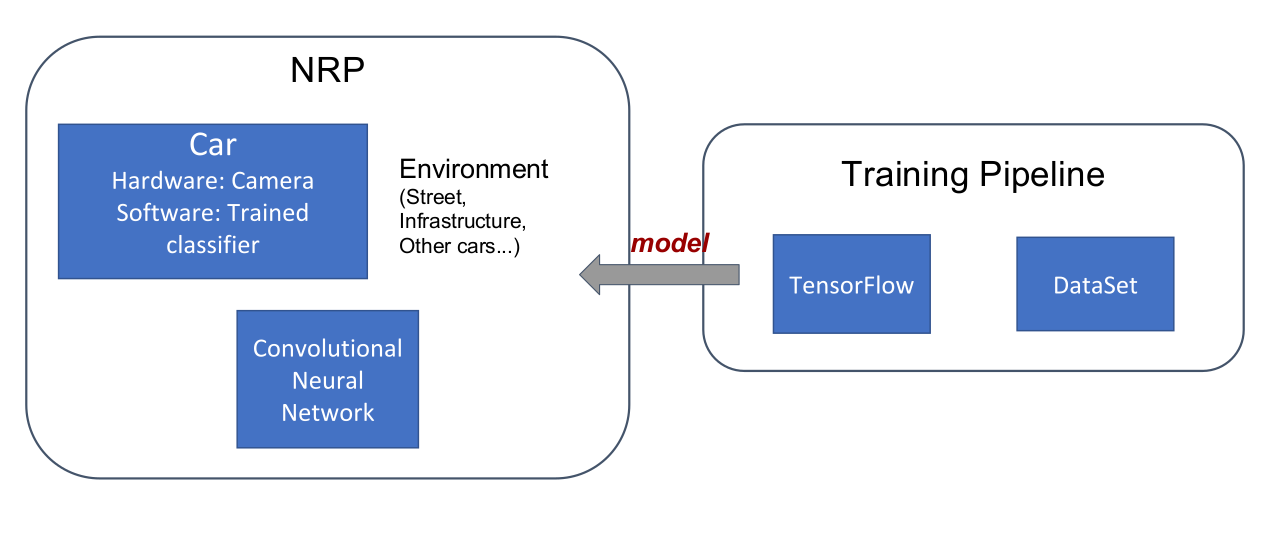
\includegraphics[width=0.9\textwidth]{chapter/images/img-1.png}
  \caption{Architecture of the NRP traffic sign detection for autonomous driving}
  \label{fig:img}
\end{figure}


The implementation part will be described as follows: 
\begin{itemize}
	\item Traffic signs detection
	\item Car control
	\item Traffic signs
	\item Environment setup: street and car model
	 
\end{itemize}

\subsection{Detection of Traffic Signs}

To implement the detection of traffic signs a neural network model was trained. Training was performed on pre-trained model from the tensorflow object detection models zoo, namely ssdlite mobilenet v2 model pre-trained on COCO dataset\cite{DBLP:journals/corr/HuangRSZKFFWSG016}. MobileNets family of computer vision models is designed for resource constraint environments while maintaining high accuracy. They target mobile and embedded devices, their careful use of resources allows us to achieve satisfactory inference speed when running the detection in NRP, which does not support the use of graphics processing units at the moment. The model also implements SSDLite framework, which is a mobile friendly version of the regular SSD framework\cite{DBLP:journals/corr/abs-1801-04381}. This use of multibox detector method allows the model to perform localization of objects, which allows us to get the bounding boxes of the traffic signs. 


The dataset for training was fully generated without using existing traffic signs datasets. One image per each traffic sign used in the experiment was pasted on backgrounds, which were images randomly drawn from the COCO dataset. By providing sufficiently many and diverse images (not semantically related to the traffic scenes) we attempt to make our model generalize well in any environment. 3000 (three thousand) images per each traffic sign was generated as well as automatically produced annotation, which contained the class of the image and location of the traffic sign in the image by providing x coordinate minimum and maximum and y coordinate minimum and maximum. To make the detection more robust several random modifications were applied to signs in each image, such as perspective deformation, brightness change, blur and noise. In \ref{fig:img} we can see an example of one image from a total of 9000 images dataset.

\begin{figure}
  \centering
  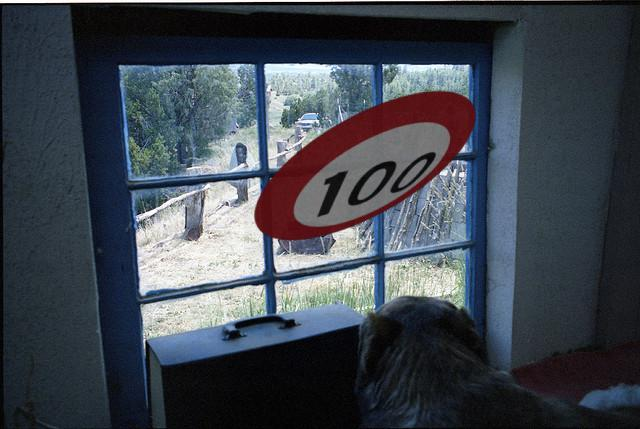
\includegraphics[width=0.7\textwidth]{chapter/images/img-2.jpg}
  \caption{Example of an image generated to train the neural network model}
  \label{fig:img}
\end{figure}


After training was performed several model checkpoints were tested in NRP and the best performing model was selected by simple observation of the performance. The current version of the model was achieved at step 18999 with the batch of 16 images, which is less than 37 epochs. The batch size was constrained by the GPU's memory on the personal computer used for training. Hyperparameters such as learning rate were used from the default training configuration from the tensorflow object detection api. Training script and config file, as well as dataset generation script will be submitted as a project deliverable. 8 percent of images were used as validation set, breaking down the 9000 images into 720 images validation and 8280 images training set.


Inference graph was saved in the .opt/graph\_def directory of the NRP container as well as accompanying label map. The training was performed using tensorflow and the transfer function of our experiment makes use of tensorflow api. Object detector transfer function runs a tensorflow session, which returns the number of detections in an image it gets from the car's camera, scores for these detections, classes and boxes, where boxes are maximum and minimum x and y coordinates of the detected traffic signs. Afterwards the square of the bounding box for each detection is calculated to determine, which of the signs has the biggest bounding box, assuming that this sign is the closest one to the car. After such sign is determined it is passed to the car's transfer function, where the car's logic is implemented. 

\subsection{Car Control}
The car is set to drive straightly forward at a constant speed at its original state. When traffic signs come into the camera view, the closest sign determined by our neural network will be passed to the transfer function by a global map variable. According to the output of the detection process, the transfer function will return a "Twist" message, which contains a vector describing the three-dimensional linear velocity and a vector describing the three-dimensional angular velocity. This message will then published to the ROS topic "/husky/cmd\_vel" and the desired velocity will be applied by the car. The car has a base speed coefficient, which is modified in response to the detected sign. The car can accelerate/decelerate and stop. The speed level is maintained until the car detects another sign.


\subsection{Speed Limit Signs}

The traffic sign model in the experiment is the most important part of the environment as it directly influences the car’s decision making. For the simplicity, only speed limit signs are to be used because this sign can already lead to a visible effect (acceleration or deceleration) on the car. The traffic sign cognition function of the car can therefore be obviously proved. 



The technique used in the car to recognize the traffic sign is neural network. And the training dataset of the neural network is a fully generated dataset. As this dataset doesn’t include all types of speed limit signs, the model should include the right speed limit model (rather than a random one) so that the trained model in the car can detect and recognize the speed limit sign in the right way. In the experiment, speed limit signs for 100 km/h and 20 km/h are used.



A compatible model in NRP is defined mainly by three files: ``limit20.dae'', ``model.config'', and ``model.sdf''. The ``model.config'' file configures the author, model name, model version and description. The ``model.sdf defines'' the physical property of the model like geometry and collision property. The ``limit20.dae'' specifies the property of the speed limit sign in detail. For example, texture, material, and relative position of the traffic signs are defined in this file.



To speed up the model building, a reference model in ``.skp'' format is downloaded from the internet. To change it into a ``.dae'' format which is compatible with NRP, the 3D modeling software ``Sketchup'' in operating system Windows 10 (this software is not supported in Ubuntu) is used to convert the file to ``.dae'' format. The following operations are implemented in Ubuntu 16.04 operating system. 



After having the above files, the scripts are edited according to the model physical property, model name, model directory, and reference pictures. A new ``.sdf'' file is created to configure the geometry, link, collision property with the use of the ``.dae'' file. 

After implementing the above steps, the model should be available in the NRP platform.

\subsection{Straight Road Section}

Currently no urban road models are available in the NRP model library. To make a vivid street model and thus improve the simulation visual quality, a road model is needed. The main requirement on the road model is that it should be able to support objects on it. Since the car calculates it's motion in the simulation world, the road need to be flat enough to avoid any unpredictable behaviors of the car. NRP models like large concrete ground and carpet are referenced to make the road model.


The road model consists of four files: model.config, model.sdf, road.dae, road.png. Since NRP is partly based on Gazebo, the model structure is quite similar to the gazebo model. A gazebo model has three levels: 3D object, model, world. NRP model is quite similar to this structure. 


The road model starts from a 3D object, which is defined in "road.dae". Important information such as geometry and texture of the road is defined in this file. The image road.png is referenced in road.dae as texture of road surface. The geometry section has three main sources: mesh position, mesh normals, mesh map. To build our road model based on the large concrete ground, we have adjusted some values in these sources. For example, the large concrete ground has 9 sections, while we only need 3 sections to make a road. So mesh positions need to be changed. As for the texture, the dae file has a complex structure. The image is imported as library\_images in road.dae. It is then used in library\_effects. In the next step, it makes library\_materials. Finally materials is apply to the model. 


"model.sdf" is the bridge between a 3D model and a gazebo model. This file imports the 3D model "road.dae", defines its initial position, collision and visual property. The road model is now a complete module and can be used in NRP platform. This is the level of Gazebo model. A street environment corresponds to world level in Gazebo, which will be explained in the next section.

"model.config" defines descriptions of the model and author. The information is not relevant for running simulations. 

\subsection{Street Environment Setup Section}
The street scene consists of three parts. A long straight road, traffic signs at the side of the road, background.

After opening an experiment, we cleared the environment and built our street scene. We imported three roads into the environment. Limit100, limit20, stop signs are placed consequently along the road. The car starts in front of limit100 as a high speed, when it percepts the limit100 sign, is slows down to follow the traffic rule. Afterwards it percepts limit20 and slows down again. It will stop when it sees the stop sign. So three signs are arranged in this order.


We put three large concrete ground models below road and traffic signs. This is only for the visualization. Because the road has collision property and can support the car. A sun light model is also added into the environment. Otherwise the street would be dark everywhere.

We also encountered a problem when we run our car on the road. The car wouldn't follow straight lines. The reason was the friction between road and wheels of the car. They both used ode engine to calculate friction. Parameters mu and mu1 control the contact force. So parameters in the model are modified to keep the car on a straight line. 

After setting up all the environment, we downloaded the world model so that we can use it later.


\begin{figure}
  \centering
  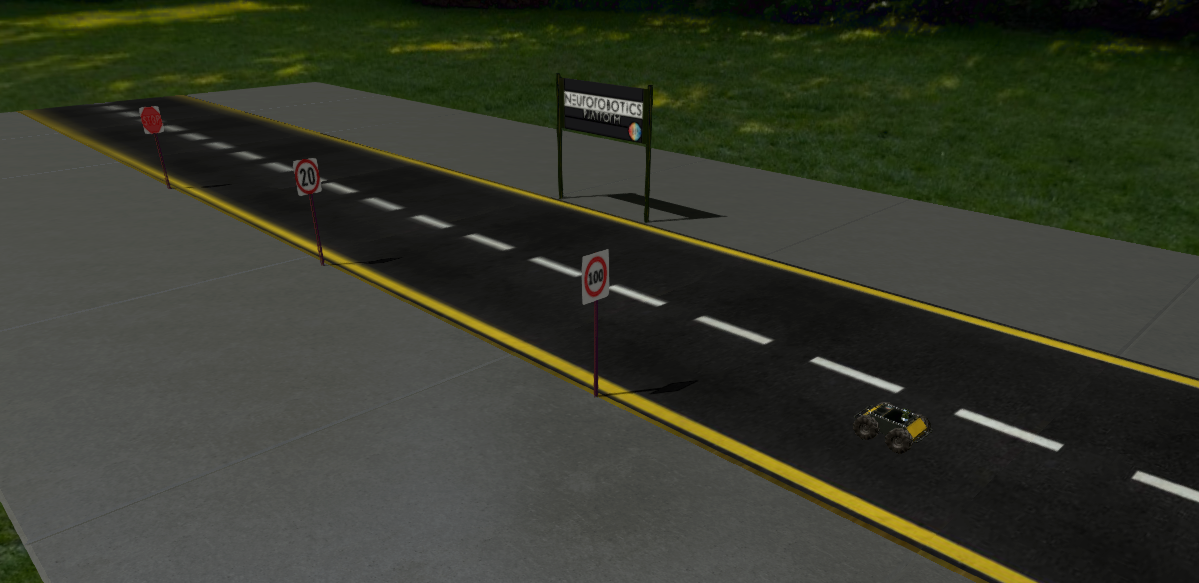
\includegraphics[width=0.9\textwidth]{chapter/images/img-3.png}
  \caption{A sreenshot of the environment in the traffic sign detection experiment}
  \label{fig:img}
\end{figure}


\subsection{Robot Setup Section}

We used husky model in our experiment. To set up the hardware part of the car, three steps are performed.


Firstly, modify parameters of the husky model in the NRP. As mentioned in the last section, the friction plays an important role in the robot motion. Since the friction parameter of this car is already large enough, we increased the mass of the car so that it has a tight contact with the road.


Secondly, import the robot model in TrafficSignsProject.bibi in the experiment directory. That's where we define which robot to use.


Finally, define the initial position of the robot in TrafficSignsProbject.exc. The car should be placed above the road and fall down to the road. Otherwise, it has the risk of being stuck in the road.



